\section{The Trip Itinerary Planning Problem}
\label{sec:problem}

We now introduce the \emph{Trip Itinerary Planning (TRIP) Problem}.
We assume a city with different points of interest (POIs),
represented as a graph where each POI is a node.  Every pair of POIs
is connected by multiple edges that represent the mode of transport
from one POI to the other.  Thus, if there are two modes of
transport, say, walking and taxi, there will be two edges between every
pair of POIs.  The weights on an edge $e$ is a tuple $\langle t^{m}_e,
c^{m}_e \rangle$ that represent the time of travel and the cost of travel
respectively for the particular travel mode $m$ selected.  The time of travel is
typically measured using a constant speed.  Thus, the distance
between the pair of POIs is divided by the constant speed to convert it
to time.  Similarly, the taxi cost is computed using a fixed formula
on the distance.  For walking, the cost is $0$.  Each POI $v$ has a
tuple $\langle t_v, c_v, U_v \rangle$ associated with it that
represents the time it takes to visit the POI, the cost (entry fees,
etc.) and the utility a traveler gets by visiting the POI
respectively.  While the
time to visit may change from one traveler to another, in this work,
we keep this fixed as the average time.  We do, however, let the time of visit of a POI
vary for a user, with the associated
utility also changing.  Additionally, a POI may have a feasible
time-interval of visit in a day (say, a sunset spot, which can be
visited only in the afternoon from 4-6 pm), beyond which visiting it
gives a utility of $0$.  Each POI is also marked with a category or type (e.g.,
park, museum, etc.).  Finally, we have a total time budget and a cost
budget.  Both the time and the cost budgets are spent in traveling as
well as visiting the POIs.  The objective of the \emph{TRIP} problem
is to \emph{find an itinerary}, i.e., a sequence of POIs, that
\emph{maximizes the total utlity} of visiting the POIs under the
given time and cost budget.  The itinerary is prepended by a source
point (e.g., a hotel or an airport) and appended by a destination
point (again, hotel, airport, etc.).  The time and cost to travel
from the source to the first POI and from the last POI to the
destination has to be also taken into account.

\begin{figure}[t]
	\centering
    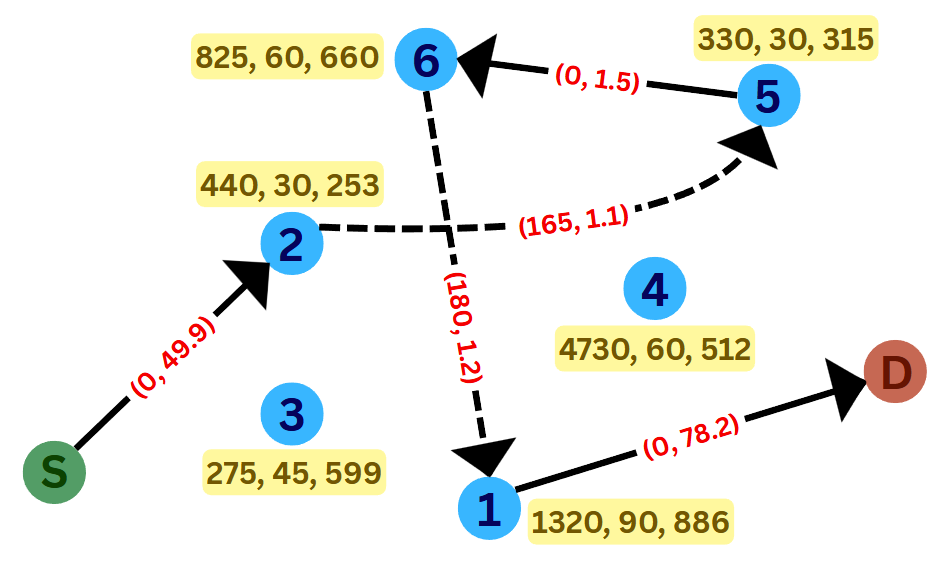
\includegraphics[width=0.75\columnwidth]{plots/updatedExample.png}
	\figcaption{Example of an optimal itinerary (solid edges represent walking and dashed edges represent taxi; edge labels depict \{travel cost, travel time\} while vertex labels depict \{visit cost, visit  time, utility\}; S and D are source and destination)}
	\label{fig:example_graph}
\end{figure}

\begin{table}[t]
	\centering
	\resizebox{0.85\columnwidth}{!}
	{
		\begin{tabular}{c l rrr}
			\toprule
			\textbf{ID} & \textbf{Category} & \textbf{Visit Time} & \textbf{Utility} & \textbf{Visit Cost} \\
			\midrule
			%S & Source      & 0  & 0   & 0    \\
			1 & Park        & 90 & 886 & 1320 \\
			2 & Park        & 30 & 253 & 440  \\
			3 & Park        & 45 & 599 & 275  \\
			4 & Museum      & 60 & 512 & 4730 \\
			5 & Museum      & 30 & 315 & 330  \\
			6 & Museum      & 60 & 660 & 825  \\
			%D & Destination & 0  & 0   & 0    \\
			\bottomrule
		\end{tabular}
	}
	\tabcaption{Details of Points of Interests (POIs)}
	%\vspace*{-4mm}
	\label{tab:example_poi}
\end{table}

An itinerary $I$ of $n$ POIs is, thus, represented as a sequence
%
\begin{align}
	I = [ S, v_1, \dots, v_n, D ]
\end{align}
%
The total time spent for itinerary $I$ is
%
\begin{align}
	t(I) = \sum_{\forall m} t^{m}_{S,v_1} + t_{v_1} + \sum_{\forall m} t^{m}_{v_1,v_2} + t_{v_2} + \dots \notag \\ + \sum_{\forall m} t^{m}_{v_{n-1,v_n}} + t_{v_n} + \sum_{\forall m} t^{m}_{v_n,D}
\end{align}
%
which takes into account both the travel time and visiting time.  Similarly,
the total cost of itinerary $I$ is 
%
\begin{align}
	c(I) = \sum_{\forall m}c^{m}_{S,v_1} + c_{v_1} + \sum_{\forall m}c^{m}_{v_1,v_2} + c_{v_2} + \dots \notag \\ + \sum_{\forall m}c^{m}_{v_{n-1,v_n}} + c_{v_n} + \sum_{\forall m}c^{m}_{v_n,D}
\end{align}
%
which again takes into account both the travel cost and visiting cost.  The
utility obtained from $I$ is
%
\begin{align}
	U(I) = U_{v_1} + U_{v_2} + \dots + U_{v_n}
\end{align}
%
Given a time budget $T$ and a cost budget $C$, the TRIP problem is to find the
itinerary $I$ that maximizes $U(I)$ subject to the budget constraints:
%
\begin{align}
	& \arg\max_I U(I) \\
	\text{subject to } & t(I) \leq T \text{ and } c(I) \leq C
\end{align}

The traveler may put additional constraints on the itinerary such as
a particular POI must be visited (e.g., Eiffel Tower in Paris).  She
may also put restrictions in the form that not more than $k$ POIs of
the same category may be included and/or at least one POI of a particular
category must be included, etc.  She may also put in ordering
constraints, such as a temple must be visited before a museum, etc.  The feasible itinerary $I$ must satisfy all these
constraints.

Consider an example of a city that has 6 POIs.
Table~\ref{tab:example_poi} shows the various time and cost values for
the POIs while Table~\ref{tab:example_walk} and
Table~\ref{tab:example_taxi} shows the travel times among the POIs and
the source and destination marked by $S$ and $D$ respectively for
walking and taxi respectively.

\begin{table}[t]
	\centering
	\resizebox{\columnwidth}{!}
	{
		\begin{tabular}{c|cccccccc}
			\toprule
			\textbf{From$\backslash$To} & \textbf{S} & \textbf{1} & \textbf{2} & \textbf{3} & \textbf{4} & \textbf{5} & \textbf{6} & \textbf{D} \\
			\midrule
			\textbf{S} & --    & 28.7  & 49.9  & 55.5  & 68.9  & 126.6 & 117.2 & 102.9 \\
			\textbf{1} & 28.7  & --    & 3.3   & 3.2   & 4.3   & 10.1  & 9.3   & 78.2  \\
			\textbf{2} & 49.9  & 3.3   & --    & 5.7   & 2.7   & 8.0   & 6.9   & 94.3  \\
			\textbf{3} & 55.5  & 3.2   & 5.7   & --    & 5.0   & 9.9   & 9.6   & 47.4  \\
			\textbf{4} & 68.9  & 4.3   & 2.7   & 5.0   & --    & 5.8   & 5.0   & 74.7  \\
			\textbf{5} & 126.6 & 10.1  & 8.0   & 9.9   & 5.8   & --    & 1.5   & 98.5  \\
			\textbf{6} & 117.2 & 9.3   & 6.9   & 9.6   & 5.0   & 1.5   & --    & 102.4 \\
			\textbf{D} & 102.9 & 78.2  & 94.3  & 47.4  & 74.7  & 98.5  & 102.4 & --    \\
			\bottomrule
		\end{tabular}
	}
	\tabcaption{Walking travel time matrix}
	\label{tab:example_walk}
\end{table}

\begin{table}[t]
	\centering
	\resizebox{0.97\columnwidth}{!}
	{
		\begin{tabular}{c|cccccccc}
			\toprule
			\textbf{From$\backslash$To} & \textbf{S} & \textbf{1} & \textbf{2} & \textbf{3} & \textbf{4} & \textbf{5} & \textbf{6} & \textbf{D} \\
			\midrule
			\textbf{S} & --    & 3.8  & 6.7  & 7.4  & 9.2  & 16.9 & 15.6 & 13.7 \\
			\textbf{1} & 3.8   & --   & 0.4  & 0.4  & 0.6  & 1.3  & 1.2  & 10.4 \\
			\textbf{2} & 6.7   & 0.4  & --   & 0.8  & 0.4  & 1.1  & 0.9  & 12.6 \\
			\textbf{3} & 7.4   & 0.4  & 0.8  & --   & 0.7  & 1.3  & 1.3  & 6.3  \\
			\textbf{4} & 9.2   & 0.6  & 0.4  & 0.7  & --   & 0.8  & 0.7  & 10.0 \\
			\textbf{5} & 16.9  & 1.3  & 1.1  & 1.3  & 0.8  & --   & 0.2  & 13.1 \\
			\textbf{6} & 15.6  & 1.2  & 0.9  & 1.3  & 0.7  & 0.2  & --   & 13.7 \\
			\textbf{D} & 13.7  & 10.4 & 12.6 & 6.3  & 10.0 & 13.1 & 13.7 & --   \\
			\bottomrule
		\end{tabular}
	}
	\tabcaption{Taxi travel time matrix}
	\label{tab:example_taxi}
\end{table}

Suppose a traveler has a time and cost budget of $360$ minutes and $3500$ units respectively.
Additionally, she puts in the contraints that (1)~POIs 1 and 2 must be visited, (2)~POI 2 must be visited before POI 1, and (3)~POI 3, if visited, must be before both POI 2 and POI 5 (if visited).
Further, she must visit at least 2 POIs of the category Park, and will not visit more than 2 POIs of the category Museum.

Respecting all these constraints, the optimal itinerary is $[S, 2, 5, 6, 1, D]$, as shown in Fig.~\ref{fig:example_graph}.  Note that the
POIs 3 and 4 were not included.  The total utility obtained from the
itinerary is $2114$ units, and the time and cost spent 
are, respectively, $341.9$ minutes and $3260$ units.

